% !TEX root =../thesis.tex
\chapter{Introduction}
\label{chap:intro}

\lettrine[lines=4]{F}{or} millenia mankind has watched and studied the nightsky. Apart from planets and comets it appeared an immuatble canvas on which the stars rested. It comes as no surprise that for ancient civilizations supernovae (which were very rare events, occuring only every few centuries ) were interpreted as important Omens as they broke the paradigm of the unchanging nightskies. As these events are so rare their origin remained a mystery until the middle of the last century \citet{1934PNAS...20..254B} suggested that "the phenomenon of a super-nova represents the transition of an ordinary star into a body of considerably smaller mass". For the last 85 years the "supernova-branch" in astronomy has been developing. There have been many advances, but there are still very unknowns about supernovae. This work addresses two subfields of supernovae: The unsolved progenitor problem for Type Ia Supernovae as well as quantifying the nucleosynthetic yield of Type Ia supernovae from low-resolution spectra.


\section{Ancient Supernovae}
\label{sec:ancientsn}

One of the earliest recorded supernovae is SN185. It first appeared in December of 185 and was visible (however fading) till the August of 187. The main record is the \textit{Houhanshu} \citep{2006ChJAA...6..635Z} which had a described it to be close to $\alpha$ \textit{cen}. Follow-up in modern times have revealed a supernova remnant in a distance of roughly 1\;kpc near the $\alpha$ \textit{cen} \citep{2006ChJAA...6..635Z}. SN185 is often named as the oldest written record of a supernova, this is however sometimes contested as it is still not completely clear if the so called "guest star" was a comet or a supernovae. 

The oldest undisputed record of a supernova is SN1006. It was observed worldwide by asian, arabic and european astronomers. 
mention 1885 in andromeda\cite{1885AN....112..360H}


\section{Modern supernova observations and surveys}
\label{sec:}
The most famous and often quoted paper is \citet{1934PNAS...20..254B}. It termed the term supernova and established the difference between common novae and supernovae. \citet{1934PNAS...20..254B} suggested that these luminous events are caused by the death of stars. 

In order to understand the phenomenon of the supernova better Zwicky began a supernova search with the 18-inch Schmidt telescope. He found several supernovae cite?? which in turn inspired Minkowski to classify these supernovae by their spectra \citet{1941PASP...53..224M}. 
He categorized the 14 known objects into two categories. Those without hydrogen he called 'Type I', those with hydrogen he called 'Type II' (see section \ref{sec:sn_classification} for a more detailed description).

With the advent of affordable computing in the 1960s the first computer controlled telescopes were build. The 24-inch telecope was built by the Northwestern University and was deployed in Corralitos Observatory in New Mexico. This search resulted 14 supernovae. 

The 1990's can be described as the decade of the supernova surveys. The Leuschner Observatory Supernova Survey began in 1992 followed shortly by the Berkeley Automatic Imaging Telescope (BAIT). These searches resulted in 15 supernovae by 1994 \citep{1994AAS...185.7905V}. One of the most well known discoveries is SN 1994D. This supernovae was observed with the Hubble Space Telescope and resulted in an image that is widely used today (see Figure \ref{fig:sn1994d}).

These successful programmes were succeeded by the Lick Observatory Supernova Search (LOSS) using the Katzman Automatic Imaging Telescope (KAIT). By the year 2000 it had found 96 supernovae \citep{2001ASPC..246..121F}.


\section{Supernova classification}
\quote{Gallia est omnis divisa in partes tres.}

\label{sec:sn_classification}
The classification of supernovae started in the 1941 when Minkowski realized that there seem to be two main types \citep{1941PASP...53..224M}. Minkowski relied on optical low-resolution spectra near the maximum to identify the two main subtypes (see Figure \ref{fig:sn_spectra_turatto} for an overview of spectra of different types). Those containing a hydrogen line (6563 \AA) he called Type II supernovae and those showing no hydrogen he called Type I supernovae.  

\begin{figure}[htbp] %  figure placement: here, top, bottom, or page
   \centering
   \includegraphics[width=\textwidth]{chapter1/plots/sn_classification.pdf} 
   \caption{}
   \label{fig:sn_classification}
\end{figure}

This basic classification has remained to this day, however the two main classes branched into several subtypes.
During the 1980s the community discovered that most \sneia\ showed a broad Si II line at 6130 \AA, but that there was a distinct subclass of objects that lacked this feature. These Silicon-less objects were then subclassed further into objects that showed helium -- now known as Type Ib --  and those that did not were called Type Ic \citep{1987ApJ...317..355H, 1986ApJ...306L..77G}. The classical Type I supernova was renamed to Type Ia (see Figure \ref{fig:sn_classification}). 

\begin{figure}[htbp] %  figure placement: here, top, bottom, or page
   \centering
   \includegraphics[width=\textwidth]{chapter1/plots/sn_class_spectra.pdf} 
   \caption{example caption}
   \label{fig:sn_class_spectra}
\end{figure}

This classification only uses static spectral features. In recent years, however, there has been a push towards also using the lightcurve and spectral evolution as classification parameters. \citet{2005ApJ...623.1011B} provide an overview of this subclassing of \sneia\ and suggest that there are two distinct subclasses of \sneia. As a parameter for this further partitioning they use the velocity measured from the Si II feature at 6355 \AA. Those with a relatively fast decline in this radial velocity they call \hvg\ (high velocity gradient) those with a slow decline rate are named \lvg\ (low velocity gradient). 
Figure \ref{fig:sn_class_lvg_hvg} shows the velocity gradient of 26 supernovae taken from  \citet{2005ApJ...623.1011B}

\begin{figure}[htbp] %  figure placement: here, top, bottom, or page
   \centering
   \includegraphics[width=\textwidth]{chapter1/plots/velocity_gradient.pdf} 
   \caption{example caption}
   \label{fig:sn_class_lvg_hvg}
\end{figure}

Futhermore there seems to be also a split in the intrinsic luminosity of \sneia. The canonical objects for these distinct brightness classes are the overluminous 1991T \citet{1992AJ....103.1632P} and the faint 1991bg .
Faint supernovae are fast decliners both in velocity as well as luminosity \citet{2005ApJ...623.1011B}. The bright supernovae seem to occur in both the \hvg\ and \lvg\ group. I will discuss the physical implications of these two subtypes in section \ref{sec:snia_physics}.

In summary, although there are several different subclasses the \snia as a class itself is relatively homogenous when compared to the different \sneii. ??? rates????

\begin{figure}[htbp] %  figure placement: here, top, bottom, or page
   \centering
   \includegraphics[width=\textwidth]{chapter1/plots/snii_lc_comparison.pdf} 
   \caption{example caption}
   \label{fig:snii_lc_comparison}
\end{figure}
\sneii span large ranges in observables like luminosity, explosion energies, etc. We can divide the main class into three main subclasses Type II Plateau \citet[\sniip][]{1979A&A....72..287B} which have a relatively flat light curve after an initial maximum (see Figure \ref{fig:sniil_sniip}), in contrast the Type II Linear \cite[\sniil][]{1990MNRAS.244..269S} has a rapid linear decline after the maximum. The third subclass is the narrow-lined \snii (\sniin) which is characterized by narrow emission lines, which are thought to come from interaction with the \csm. Unlike the \sneia there are numerous intermediate objects among these three basic classes. 

???? 

For a more comprehensive review of the classification of supernovae the reader should consult \citet{2003LNP...598...21T, 2007AIPC..937..187T}.

\section{Core Collapse Supernova}
\subsection{Observation}

\subsection{Theory}
All \snii are believed to be powered by the collapse of the electron-degenerate iron core of massive stars. For the iron core to form there had to be several prior stages of evolution.

\paragraph{Evolution of Massive Stars:}  To understand the state of the star shortly before supernova evolution it is imperative to follow its evolution. For the topic of \snii we will concentrate on the nuclear physics issues of massive star evolution in this section. In the scope of this work we will follow a single massive star as a progenitor. There has been ample of suggestions that \snii progenitors are binary, but their evolution is much more complex and is outside the scope of this work?? citation needed??.  In this context massive stars are stars bigger than 8 \msun. This is the minimum mass for a star that is believed to explode in a \snii. Like all stars massive stars spend most of their lives on the main-sequence burning hydrogen. This happens via the carbon-nitrogen-oxygen cycle and its various side-channels (e.g $^{12}C(p,\gamma)\rightarrow^{13}N(e^+\nu)\rightarrow^{13}C(p,\gamma)\rightarrow^{14}N(p,\gamma)^{15}O(e^+\nu)\rightarrow^{15}N(p,\alpha)\rightarrow^{12}C$). For a 20 \msun star this phase lasts for 8.13 \myr (see \citet{2002RvMP...74.1015W}).

As the star evolves it begins to ignite Helium which burns via the triple-$\alpha$ process to Carbon ($3\alpha\rightarrow^{12}C$) and then to Oxygen ($^{12}C(\alpha,\gamma)\rightarrow^{16}O$). Table 1 in \citet{2002RvMP...74.1015W}) lists 1.17 \myr\ for this phase. 

Due to neutrino losses the stellar evolution is qualitatively different after helium burning. A neutrino-mediated Kelvin-Helmholtz contraction of the carbon-oxygen core describes the advanced stages of nuclear burning in massive stars well (\citet{2002RvMP...74.1015W}). This is contraction is occasionally delayed when the burning of new fuel sources counter-acts the neutrino losses. The star in the end is composited of a series of shells that burn the above fuel and deposit the ashes on the shell below (see Figure \ref{fig:fusion_shells}). There are four distinct burning stages. Their principal fuels are carbon, neon, oxygen, magnesium and silicon.

\begin{figure}[htbp] %  figure placement: here, top, bottom, or page
   \centering
   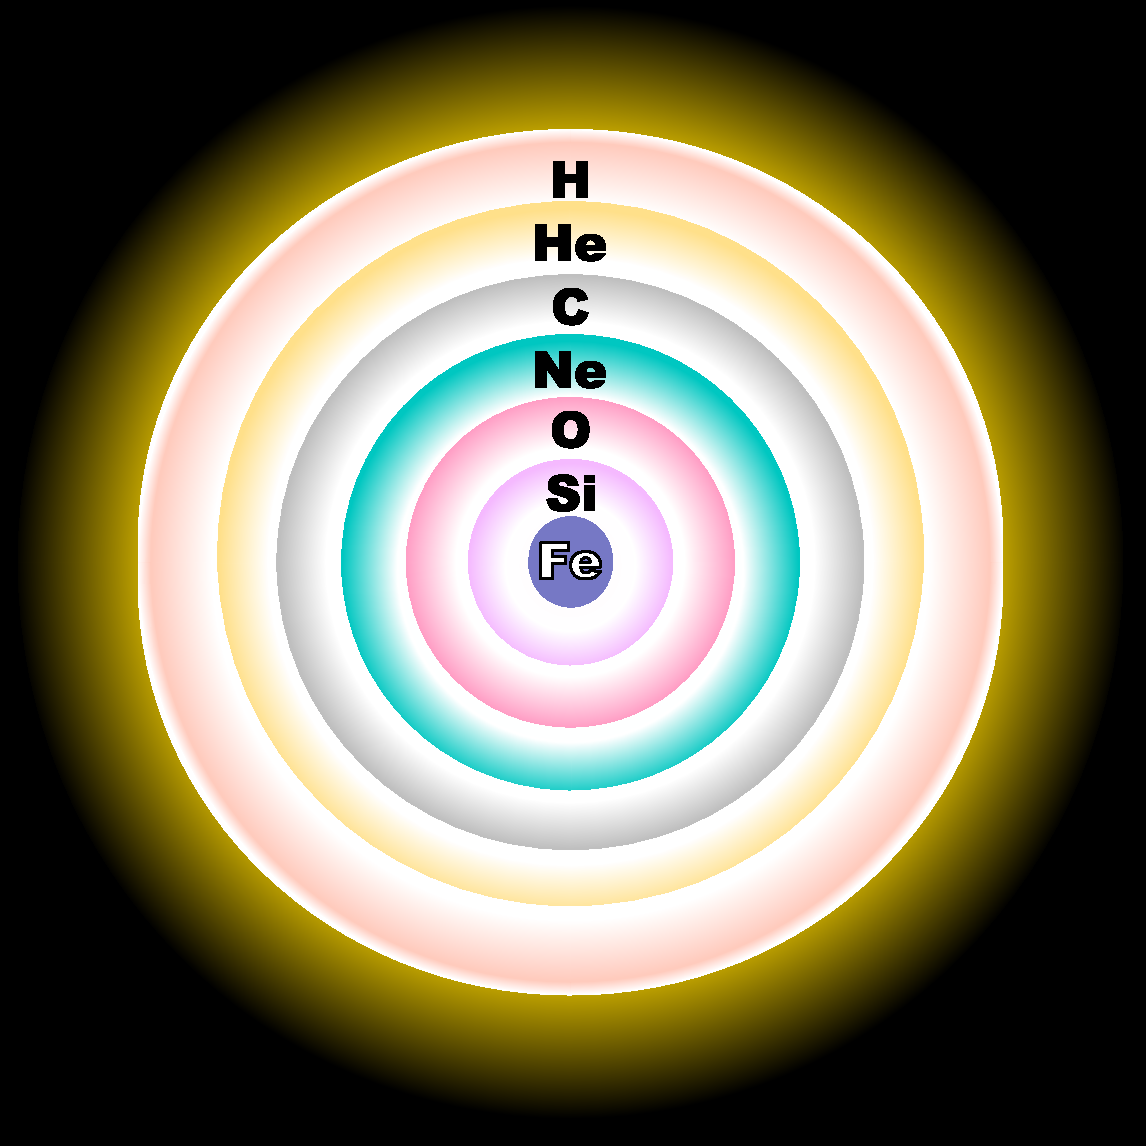
\includegraphics[width=\textwidth]{chapter1/plots/fusion_shells.pdf} 
   \caption{example caption}
   \label{fig:fusion_shells}
\end{figure}


In the carbon burning stage two $^{12}$C nuclei are fused to an excited state of Magnesium which then decays slowly to $^{23}$Na (see \ref{eqn:c_burning}).
\begin{eqnarray}
^{12}C+^{12}C\rightarrow^{24}Mg&\rightarrow&^{23}Mg+n \nonumber \\
	&\rightarrow&^{20}Ne + \alpha \nonumber \\
	&\rightarrow&^{23}Na +p \nonumber \\
	\label{eqn:c_burning}
\end{eqnarray}

Although oxygen has a lower Coulomb barrier, the next nucleus to burn after Carbon is Neon. This layer is composed of of  $^{16}$O, $^{20}$Ne and $^{24}$Mg and burns Neon with high-energy photons from the tail of the Planck distribution ($\rm ^{20}Ne(\gamma,\alpha)^{16}O$). 

Going down one shell, one has now a composition of mainly $^{16}$O, $^{24}$Mg and $^{28}$Si. The bulk nucleosynthetic reaction is shown in \ref{eqn:c_burnin}. 

\begin{eqnarray}
^{16}C+^{16}O\rightarrow^{28}Si&\rightarrow&^{31}S+n \nonumber \\
	&\rightarrow&^{31}P + p \nonumber \\
	&\rightarrow&^{30}P + d \nonumber \\
	&\rightarrow&^{28}Si + \alpha \nonumber \\
	\label{eqn:c_burning}
\end{eqnarray}

The last shell is of burning $^{28}$Si to $^{56}$Ni is very complex. The obvious reaction $^{28}\textrm{Si}+^{28}\textrm{Si}\rightarrow^{56}\textrm{Ni}$ does not take place, but is replaced by a very complex network of isotopes to burn to $^{56}\textrm{Ni}$. In simulations this is computationally intensive and numerically unstable (e.g .  \citet{1978ApJ...225.1021W} who carry a 128-isotope network). 
Following silicon burning the composition consists of mainly iron-group nuclei. 
At the end of silicon burning we are reaching nuclear statistical equilibrium. 

\paragraph{Core collapse} Before the collapse the core, consisting of iron peak elements. Neutrino losses during carbon and oxygen burning decreased the central entropy sufficiently so that the core becomes electron degenerate. Such a degenerate core, which is higher than the Chandrasekhar mass (adjusted for Y$_e$, entropy, boundary pressure and other parameters will collapse. 

There are two main instabilities that facilitate the collapse. AS the density rises the Fermi-Energy becomes high enough for electrons to capture onto iron-group nuclei. This capture process removes electrons that were providing degeneracy pressure and reduces the structural adiabatic index. 
The second instability is the rise to temperatures where the nuclear statistical equilibrium favours free $\alpha$-particles. The collapse eventually leads to nuclear densities, the hard-core potential acts as a stiff spring during the compressive phase. It stores up energy and eventually releases this energy. The core bounces.  
\citet{1985PhRvL..55..126B,1987PhRvL..59..736B} believed the core bounce to provide the energy for the ensuing supernova explosion. More recent simulations however show that the bounce shock is not sufficient for a \snii explosion. The bounce shock looses energy by photodisintegrating the nuclei it encounters (loosing roughly $10^{51}$\,\erg\ per 0.1\,\msun). Different neutrino flavours  that the resulting neutrino winds likely play a big role. 

The energy for a successful explosion is now thought to come from neutrino energy deposition. This reinvigorates the shock and leads eventually to an explosion which ejects the envelope of the massive star. A newly born neutron star is left behind.

The precise explosion mechanism is unknown. Using progenitor models with different parameters like rotation and mass lead to different outcomes. \citet{2002RvMP...74.1015W}provide a very comprehensive review of the theory of evolution and core collapse. In particular they lay out a more extensive description of the scenarios after core-bounce.

\paragraph{Pair instability}
One explosion scenario worth mentioning is that of the pair-instability supernova. This course of events only affects stars with a helium core of more than 40\,\msun. After core helium burning the star starts to contract at an accelerated rate. The energy releases during this process is used to produce electron-positron pairs rather than raising the temperature. If significant densities are reached, oxygen fusion eventually halts the implosion and the collapse bounces to an explosion. For very high stellar masses it is believed that oxygen fusion does not provide enough energy to halt the collapse and the star becomes a black hole.

\paragraph{Type II Supernovae}
The observables of these stellar cataclysm are the light curve, spectra and for one case even the neutrino wind. The supernovae goes through three distinct phases whcih can be observed. 

The shock-breakout is the first visible signal from the supernova.  \cite{1992ApJ...393..742E} calculated a duration for the  shock breakout of SN1987A to 180\,s three minutes, its  luminosity of $5\times10^{44}$\erg\,s$^{-1}$. 
Thus far it has been observed only once in 2008D \citep{2008Natur.453..469S}. They report a duration of 400\,s with a luminosity of $6.1\times10^{43}$\erg\,s$^{-1}$.

The plateau seen in many \snii (see figure \ref{fig:snii_lc_comparison}) is produced by the recombination of hydrogen when hydrogen-rich zones cool to less than 5500\,K. The radiation comes effectively from a blackbody, whose luminosity is determined  by the radius of the photosphere.
Supernovae of Type IIL do not show this behaviour and are thus thought to have no or a very small hydrogen envelope.

After the recombination of hydrogen the light-curve drops off linearly and we see radioactivity providing the main energy source. \nififtysix decays to \cofiftysix with a half-life of 6.1\,d and then further to \fefiftysix with a half-life of 77\,d. Most of the energy of the \nififtysix decay is used to accelerated the expansion of the core. The tail of the light-curve after the plateau is mainly powered by the decay of \cofiftysix. Some light be also produced by shock interaction with the \csm.

\paragraph{Type Ib/c supernovae}
If the star lost all of it's hydrogen envelope prior to core-collapse there is no plateau visible in the light-curve. Instead the light-curve is powered by radio-active decay after shock breakout. In addition, the hydrogen lines are not visible in the spectrum. This leads to the supernova being classified as Type I. If both hydrogen and helium envelopes are lost then the supernova is classified as Type Ic. 
This loss of envelope is presumed to be caused by stellar winds or binary interactions (citation needed). 

\subsection{Gamma Ray Burst}

\subsection{Type II supernovae as cosmological probes}
\sniip have been suggested as cosmological probes by \citet{1974ApJ...193...27K}. The importance for cosmological distance probes is that the intrinsic luminosity is known well. Then a simple comparison of apparent magnitude with absolute magnitude results in a distance. At the plateau-phase of the supernova, caused by the hydrogen-recombination,  the temperature is well known(T=5000\,K). In addition it is assumed that the supernova is in free expansion, thus a measurement of the velocity and an assumption of the initial radius results in a known radius. Assuming the supernova to be a blackbody during plateau-phase one can then calculate a luminosity using the radius and the temperature. \sniip as distance candles, however, are observationally expensive and not as accurate as \snia as standard candels (15\% error for \snii  \citep{2006ApJ...645..841N} vs 7\% error for \snia).




\vspace{3cm}
nucelosynthesis
first stars
hypernovae
GRB connection
massive stars
expanding photosphere -> distance measurements
binary evoltion




\section{Type Ia Supernova}
Although known for a long time, \sneia\ have been prominently featured in astronomy in the last two decades. Their use as standard candles made the measurement of the accelerating universe possible \citep{1998AJ....116.1009R, 1999ApJ...517..565P}

\section{Observation}

\paragraph{Type Ia Supernova rates} 
The observed supernova frequency carries important information about the underlying progenitor population. The two main suggested progenitors are the single-degenerate system, in which a white dwarf accretes from an non-degenerate companion . The second suggested possibility is the merger of two white dwarfs which results in a \snia-explosion (For a more detailed explanation see Section \ref{sec:ia_progenitors}). 

\citet{1938ApJ....88..529Z} was the first work that tried to measure the supernova rate. By monitoring a large number of fields monthly, they arrived at a supernova rate by merely dividing the number of supernova detection by the number of monitoring time and galaxies. This crude method resulted in a rate of one supernova per six centuries. 

Over time many improvements were made to this first method. The rate was divided by galaxy morphological class as well as different supernova types. In addition, rates were then defined the supernova rate as number of events per century per $10^{10}$\,\lsun\ \citep[e.g.][]{1991ARA&A..29..363V,1994ApJS...92..487T}. In recent years, however, rate measurements is in relation to star formation rather than photometry (\sn\ per century per $10^{10}$\,\msun).  Therefore the community \citep[e.g.][]{2005A&A...433..807M} have switched to the use infrared photometry for the galaxy as it is thought to better represent star-formation rate then B-Band photometry \citep{2003A&A...410...83H}. 
\begin{figure}[htbp] %  figure placement: here, top, bottom, or page
   \centering
   \includegraphics[width=\textwidth]{chapter1/plots/snrates_mannucci05.pdf} 
   \caption{example caption}
   \label{fig:snrates_mannucci05}
\end{figure}

Figure \ref{fig:snrates_mannucci05} clearly shows that there is a strong connection between morphology and supernova rates. 
Both progenitor scenarios (single-degenerate and double-degenerate) suggest an "evolved" binary system. It is therefore puzzling that most supernovae occur in late-type spirals with a relative young stellar population. 
In addition, there is evidence that underluminous \sneia\ (e.g. SN 1991bg) are twice as common in late-type galaxies than in early-type galaxies \citep{2001ApJ...554L.193H}. 
Furthermore it appears that radio-loud early-type galaxies have an enhanced rate of \sneia over radio-quiet galaxies \citep{2003ApJ...587L..71D}. 

All of these factors suggest that \sneia\ can originate from two distinct progenitor scenarios and/or different explosion mechanisms \citep{1994ApJ...423L..31D,  1995ApJ...447L..69R}.

\paragraph{Light curves} Light curves are one of the most important observables. The late-time phase gave an important clue to the energy source of the light curve (radioactive decay of \nififtysix). In addition, light curves have been successfully used to calibrate \sneia as standard candles.


\begin{figure}[htbp] %  figure placement: here, top, bottom, or page
   \centering
   \includegraphics[width=\textwidth]{chapter1/plots/lightcurve_2002bo.pdf} 
   \caption{example caption}
   \label{fig:lightcurve_2002bo}
\end{figure}

The light curve can be divided in four different phases (see Figure \ref{fig:lightcurve_2002bo}). In the first phase the \sneia  rises to the maximum brightness. Although only a small fraction of \sneia have been observed in that phase. By approximating the very early phase of a \sneia with an expanding fireball it is possible to calculate that the rise is 19.5 days \citep{1999AJ....118.2675R}. The luminosity of the fireball is 
\[L\propto v^2 (t+t_\textrm{r})^2 T\,,\]
where v is the photospheric velocity, T is the temperature of the fireball, t is the time relative to the maximum and $t_\textrm{r}$ is the rise time.

The rise is very steep and the brightness increases by a factor of $\approx 1.5$ per day until 10 days before maximum. 

The \snia reaches the maximum first in the \nir roughly 5 days before the maximum in the B-Band \citep{2000MNRAS.314..782M}. 
During the pre-maximum phase the color stays fairly constant at B-V=0.1, but changes non-monotonically to B-V=1.1 30 days after maximum. 

The \snia\ starts to fade but  a second maximum is observed in the \nir \citep{2008ApJ...689..377W} ??multiple citations.  \citep{2006ApJ...649..939K} has succesfully explained this by fluorescence of iron-peak elements in the \nir. See section \ref{sec:snia_lightcurve_theory}.

At roughly 600 days after maximum the light curve begins ???? 1991t had a foreground dust??? 


Arguably the most important use of light curves is their application in normalizing \sneia\ to standard candles (see Figure \ref{fig:lsnia}). \citet[][]{1993ApJ...413L.105P} plotted the magnitude at maximum in different filters against the decline of the B-Band magnitude after 15 days (\dmb).  They found a strong linear relation with a very high correlation coefficient ($>$ 0.9). Dust extinction in the host is one of the major systematic problems and remains so to this day. 

\cite{1995ApJ...438L..17R} refined the method by using a linear estimation algorithm. This method would deliver a distance modulus by finding the offset between a template and the supernova lightcurve. They calibrated this method against a set of \sneia\ with known distances. 
Light curve fitting tools are to this day in active development \cite[e.g.][]{2007ApJ...659..122J, 2007A&A...466...11G}.

In summary, ...... see figure x



\paragraph{Spectra} Similar to light curves spectra have different phases. In the pre-maximum phase (tanaka 2010 )
polarization
\paragraph{X-Ray}

\paragraph{Radio}










\subsection{Theory}


\section{Progenitors of Type Ia Supernovae}
\label{sec:snia_progenitor}
binary evolution
chandrasekhar
white dwarfs
nucleosynthesis
iron in particular

cosmology


\section{test}




